\subsection{Experimental Setup}
\label{sec:setup}

\subsubsection{System used}

We use a server outfitted with two Intel Xeon Gold 6226R processors. Each processor comprises $16$ cores operating at $2.90$ GHz. Each core has a $1$ MB L1 cache, a $16$ MB L2 cache, and a shared L3 cache of $22$ MB. The system is set up with $376$ GB of system memory and has CentOS Stream 8 installed.\ok{}


\subsubsection{Configuration}

We employ 32-bit integers to represent vertex IDs and 32-bit floats for score computation. We utilize $32$ threads to match the system core count (unless specified otherwise). Compilation is carried out using GCC 8.5 and OpenMP 4.5.\ok{}


\subsubsection{Dataset}

The graphs used in our experiments are given in Table \ref{tab:dataset}. These are sourced from the SuiteSparse Matrix Collection \cite{suite19}. In the graphs, number of vertices vary from $3.07$ to $214$ million, and number of edges vary from $25.4$ million to $3.80$ billion. We ensure edges to be undirected and weighted with a default of $1$.


\subsubsection{Observed Graph generation}

To generate the observed graphs, we take each graph from the dataset and randomly remove $10^-4|E|$ to $0.1|E|$ edges from it --- where the endpoints of removed edges are chosen with uniformly probability.\ignore{For each batch size, we generate five random batch updates for averaging.}

\ignore{Are there no missing links in the original graphs?}

\begin{table}[hbtp]
  \centering
  \caption{List of $13$ graphs obtained SuiteSparse Matrix Collection \cite{suite19} (directed graphs are marked with $*$). Here, $|V|$ is the number of vertices, $|E|$ is the number of edges (after adding reverse edges), $D_{avg}$ is the average degree, and $|\Gamma|$ is the number of communities obtained with \textit{GVE-Leiden}.\ignore{In the table, B refers to a billion, M refers to a million and K refers a thousand.}}
  \label{tab:dataset}
  \begin{tabular}{|c||c|c|c|c|}
    \toprule
    \textbf{Graph} &
    \textbf{\textbf{$|V|$}} &
    \textbf{\textbf{$|E|$}} &
    \textbf{\textbf{$D_{avg}$}} &
    \textbf{\textbf{$|\Gamma|$}} \\
    % \textbf{$1 - \Gamma_G$} \\
    \midrule
    \multicolumn{5}{|c|}{\textbf{Web Graphs (LAW)}} \\ \hline
    indochina-2004$^*$ & 7.41M & 341M & 41.0 & 5.00K \\ \hline  % & \num{4.7e-4} & 2.9 GB
    uk-2002$^*$ & 18.5M & 567M & 16.1 & 43.1K \\ \hline  % & \num{9.6e-5} & 16 GB
    arabic-2005$^*$ & 22.7M & 1.21B & 28.2 & 3.80K \\ \hline  % & \num{5.5e-4} & 11 GB
    uk-2005$^*$ & 39.5M & 1.73B & 23.7 & 21.2K \\ \hline  % & \num{9.6e-5} & 16 GB
    webbase-2001$^*$ & 118M & 1.89B & 8.6 & 2.77M \\ \hline  % & \num{7.3e-7} & 18 GB
    it-2004$^*$ & 41.3M & 2.19B & 27.9 & 5.24K \\ \hline  % & \num{3.8e-4} & 19 GB
    sk-2005$^*$ & 50.6M & 3.80B & 38.5 & 3.75K \\ \hline  % & \num{5.8e-4} & 33 GB
    \multicolumn{5}{|c|}{\textbf{Social Networks (SNAP)}} \\ \hline
    com-LiveJournal & 4.00M & 69.4M & 17.4 & 2.33K \\ \hline  % & \num{7.9e-4} & 480 MB
    com-Orkut & 3.07M & 234M & 76.2 & 33 \\ \hline  % & \num{6.7e-2} & 1.7 GB
    \multicolumn{5}{|c|}{\textbf{Road Networks (DIMACS10)}} \\ \hline
    asia\_osm & 12.0M & 25.4M & 2.1 & 2.56K \\ \hline  % & \num{8.4e-4} & 200 MB
    europe\_osm & 50.9M & 108M & 2.1 & 3.61K \\ \hline  % & \num{6.6e-4} & 910 MB
    \multicolumn{5}{|c|}{\textbf{Protein k-mer Graphs (GenBank)}} \\ \hline
    kmer\_A2a & 171M & 361M & 2.1 & 19.4K \\ \hline  % & \num{9.4e-5} & 3.2 GB
    kmer\_V1r & 214M & 465M & 2.2 & 8.60K \\ \hline  % & \num{3.2e-4} & 4.2 GB
  \bottomrule
  \end{tabular}
\end{table}
% We convert directed graphs (marked with $*$) to undirected by duplicating edges in the reverse direction, and set the weight of each edge to $1$. and $F_{size}$ is size of the \textit{MatrixMarket} file





\subsection{Comparative Performance Evaluation}
%% Performance Comparison

In this section, we compare the performance of our approach, i.e., disregarding large hubs, and compare it with the default approach. We does this for observed graphs based on each graph in the dataset, with $10^-2|E|$ to $0.1|E|$ edges removed (the endpoints of removed edges are chosen with uniformly probability, as mentioned above), and predict the same number of edges with both approaches. For each observed graph, we predict links using the default approach, and our approach with suitable $MAX\_MEDIATOR\_DEGREE$, as identified in Section X. In Figures X, Y, and Z, we plot the runtimes, speedup, and precision respectively of only the best approach for each graph (both in terms of precision and runtime). In the figures, the labels indicate the acronyms of the similarity metric used, followed by the value of $MAX\_MEDIATOR\_DEGREE$ ($\Pi$) parameter setting (i.e., the label $HP4$ stands for the Hub Promoted similarity metric, with a $MAX\_MEDIATOR\_DEGREE$ of $4$, i.e., we avoid first order neighbors with degree greater than $4$). Note that a $MAX\_MEDIATOR\_DEGREE$ of $\infty$ is essentially the default/baseline approach. As Figures X, Y, and Z show, our approach is on average X times faster than the baseline/default approach, while predicting links with on average X\% higher precision. On the \textit{sk-2005} graph with $0.1|E|$ edges removed, our approach achieves a link prediction rate of X edges/s, and a processing rate of Y edges/s.

Although $|E^P|$ is generally unknown, an experiential and reasonable setting is  $|E^P| = 0.1 |E|$ because $10\%$ of links in the probe set are usually enough for us to get statistical solid results while the removal of $10\%$ of links will probably not destroy the structural features of the target network \cite{lu2015toward}.

\ignore{What does precision mean in the plots? \% of matching links with ground truth? How many ground truth links were missed?}

\ignore{Explain the confusion y-axis on precision.}

\ignore{Sizes of graphs are large so running other approaches (\Pi) is expensive.}

\ignore{What is the processing / prediction rate? (by predicted edges, and by number of edges in the graph)}

\ignore{Comparison with baseline approach ($\infty$), i.e., exploring all possible/reachable pairs at distance 2, and quickly computing intersection, scores, adding to heap, and merging across threads. Explain with figure in approach.}

\ignore{Why not showcase 0.01 E and 0.1 E, and remove the other plots?}

\ignore{Runtime + speedup + precision for $0.1|E|$.
Lu et al. \cite{lu2015toward} use precision.}

\ignore{Why is precision low?}
\ignore{Why precision on road networks and protein k-mer graphs low? (low average degrees)}
\ignore{It is possible that our algorithm only explores one type of connection, but the networks have various types of connections.}
\ignore{Quantifying a network's link predictability allows us to (i) evaluate predictive algorithms associated with the network, (ii) estimate the extent to which the organization of the network is explicable, and (iii) monitor sudden mechanistic changes during the network's evolution. The hypothesis of this paper is that a group of links is predictable if removing them has only a small effect on the network's structural features. We introduce a quantitative index for measuring link predictability and an algorithm that outperforms state-of-the-art link prediction methods in both accuracy and universality. This study provides fundamental insights into important scientific problems and will aid in the development of information filtering technologies \cite{lu2015toward}.}
\ignore{Are there no missing links in the original graphs?}
\ignore{Arent graphs heterogeneous? Why one method works?}
\ignore{Why do these methods perform well?}

\ignore{Can you show details plots? No.}

% Figure X shows the average runtime of link prediction with degree threshold $D$ of $4$, $8$, $16$, and $32$. Increasing $D$ increases runtime by a small amount, due to increase second-degree neighbor exploration. Increasing/decreasing the batch size however does not have an effect on runtime, as the algorithm must continue to explore possible links with higher scores even if batch/prediction size $B$ edges have been added to the prediction list. Note that runtime for link prediction with JC/HP similarity scores is nearly identical. On a batch size of $0.1 |E|$, we compare the predicted links with the links in the original graphs (without edge deletions). We observe that HP-based link prediction with $D = 16$ obtains the highest average accuracy of $2.4\%$, while HP-based link prediction with $D = 4$ obtains the highest average precision of $6.4\%$. Given the vast set of potential predictions (${}_N C_2 - |E|$), achieving high accuracy and precision remains a challenge.

\begin{figure*}[hbtp]
  \centering
  \subfigure[Runtime in seconds (logarithmic scale) for link prediction using the best similarity measure, with \textit{IHub} and \textit{LHub} approaches]{
    \label{fig:input-large--runtime}
    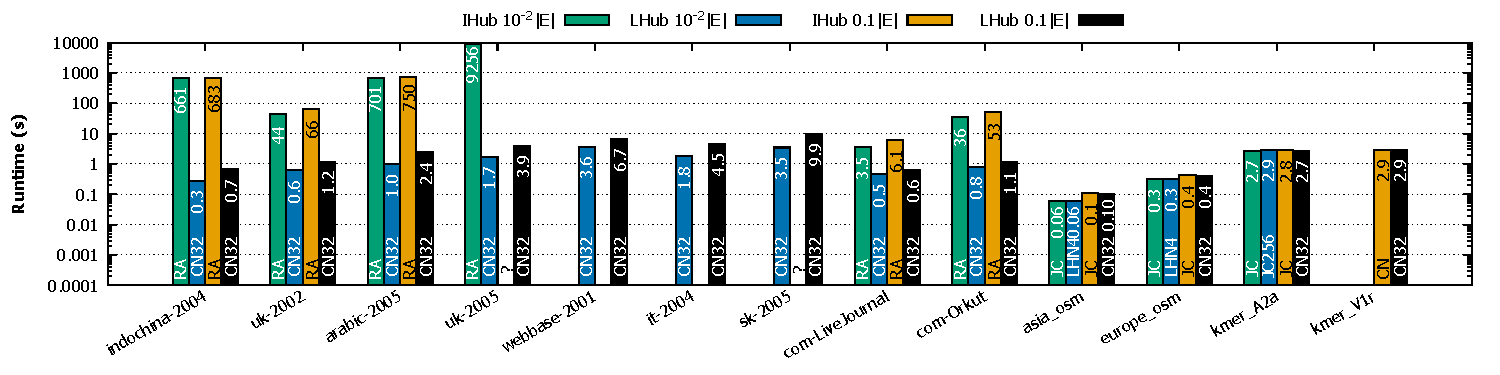
\includegraphics[width=0.98\linewidth]{out/input-large-runtime.pdf}
  }
  \subfigure[Speedup (logarithmic scale) for link prediction with the best similarity measure of \textit{LHub} approach, compared to \textit{IHub} approach]{
    \label{fig:input-large--speedup}
    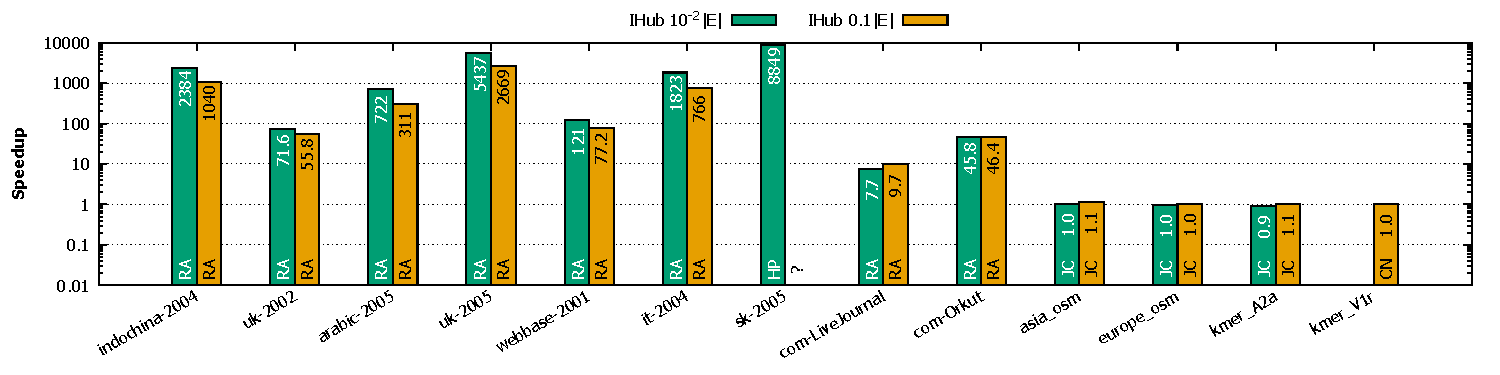
\includegraphics[width=0.98\linewidth]{out/input-large-speedup.pdf}
  }
  \subfigure[F1 score of predicted links (logarithmic scale), for link prediction using the best similarity measure, with \textit{IHub} and \textit{LHub} approaches]{
    \label{fig:input-large--f1score}
    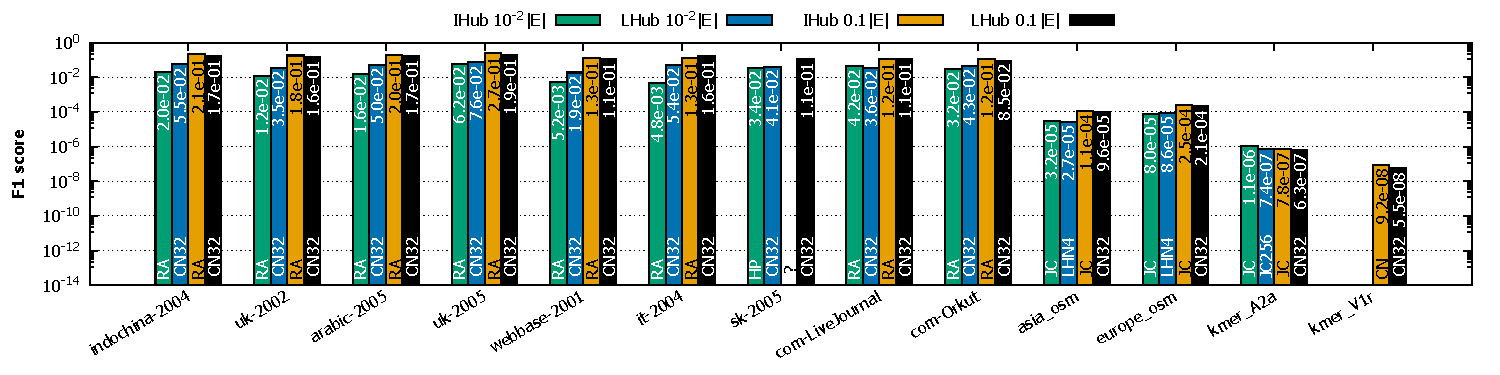
\includegraphics[width=0.98\linewidth]{out/input-large-f1score.pdf}
  } \\[-2ex]
  \caption{Runtime in seconds (log-scale), speedup (log-scale), and F1 score of predicted links (log-scale), for link prediction method using the best similarity measure, when attempting to predict $10^{-2}|E|$ to $0.1|E|$ unobserved edges $E^U$, for each graph in the dataset. For each similarity measure outlined in Section \ref{sec:metrics}, we attempt only the best hub limit $L_H$ parameter setting obtained in Section \ref{sec:select-limit} (for the \textit{LHub} approach), and then select the best among them, considering both the F1 score and runtime. Note that the numerical suffix added to the acronym of each link prediction method, with the \textit{LHub} approach, indicates the hub limit $L_H$ parameter setting.}
  \label{fig:input-large}
\end{figure*}

\begin{figure}[hbtp]
  \centering
  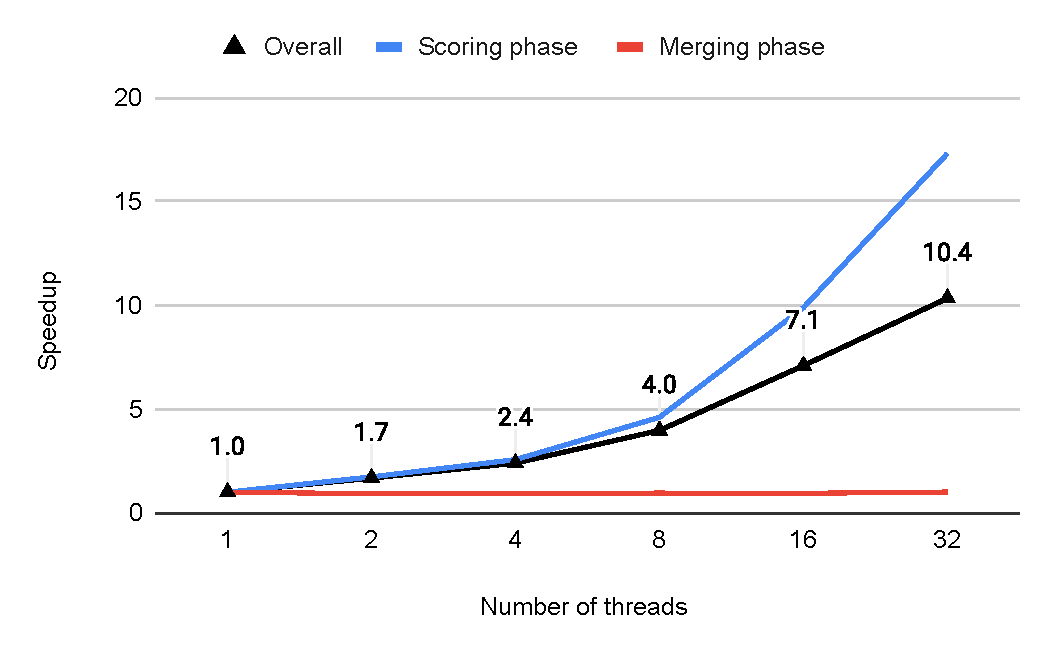
\includegraphics[width=0.98\linewidth]{out/strong-scaling-speedup.pdf} \\[-2ex]
  \caption{Overall speedup of our approach of \textit{Disregarding Large Hubs (DLH)} for link prediction, and its phases (obtaining edges with top-k scores per thread, and merging scores from each thread into a common scoreboard), with $10^{-2}|E|$ unobserved edges, with increasing number of threads (in multiples of 2). Increasing the number of threads causes work in the merging phase to increase,\ignore{thus} leading to a poor speedup.}
  \label{fig:strong-scaling}
\end{figure}





\subsection{Selecting Suitable Similarity Metric}

Extensive experiments \cite{ghasemian2020stacking} show that no known link predictor performs best or worst across all inputs \cite{zhou2021progresses}.\ignore{We expect a larger fraction of algorithms in the future studies will be designed for networks of particular types \cite{zhou2021progresses}.} In this section, we select a suitable similarity metric for link prediction for each type of graph. For this, we generate observed graphs from each graph in the dataset, such that $10^-4|E|$ to $0.1|E|$ edges are removed (the endpoints of removed edges are chosen with uniformly probability), and predict the same number of edges using the best approach for each observed graph (as identified in Section X).

In Figures X and Y, we plot the runtimes and precision of the best approach for each graph (both in terms of precision and runtime). As above, the labels in the figures indicate the acronyms of the similarity metric used, followed by the value of $MAX\_MEDIATOR\_DEGREE$ ($\Pi$) parameter setting. As Figures X, Y, and Z show, approach X is suitable for web graph. On a set of smaller graphs (not shown here), we observe that approach X is suitable for co-citation graphs.

\ignore{What does precision mean in the plots? \% of matching links with ground truth? How many ground truth links were missed?}

\ignore{Explain the confusion y-axis on precision.}

\ignore{Selecting best approach based on precision and runtime, for batch size $10^{-4}|E|$ to $0.1|E|$, and present the result. The runtime and precision of each method (appendix).}

\ignore{Sizes of graphs are large so running other approaches is expensive.}

\ignore{Why precision on road networks and protein k-mer graphs low? (low average degrees)}

\ignore{What we observe on our dataset? What we observe on smaller graphs?}

\ignore{Why the choice of best method appears to change with batch size?}





\subsection{Strong Scaling}

Finally, we assess the strong scaling performance of our optimized neighbor-based link prediction methods. In this analysis, we vary the number of thread from $1$ to $32$ in multiples of $2$ for each input graph, and measure the average time taken to predict $10^{-2}|E|$ links by Hub Promoted (HP), Leicht-Holme-Nerman (LHN), Adamic-Adar Coefficient (AA), and Resource Allocation (RA) based link prediction methods with the \textit{MAX\_MEDIATOR\_DEGREE} parameter set to $4$. The results are shown in Figure \ref{fig:strong-scaling}. It not only illustrates the overall scaling performance, but the also scaling of the two phases of each link prediction method, i.e., identifying edges with top-k scores in each thread (scoring phase), and combining the scores obtained by each thread to obtain the global top-k edges (merging phase). With $32$ threads, our optimized link prediction methods achieve an overall speedup of $7.2\times$ (with respect to sequential execution), indicating a performance increase of $1.5\times$ for every doubling of threads. The scalability is limited, as the cost of the merging phase increases with an increase in the number of threads. In fact, at $32$ threads, the merging phase obtains a speedup of $0.7\times$ (yes it is less than $1$\ignore{, as its runtime increases}), while the scoring phase achieves a speedup of $18.5\times$.

\ignore{Why is string scaling of our link prediction approach low? Why is it especially for the merging phase?}

\begin{figure*}[hbtp]
  \centering
  \subfigure[Runtime]{
    \label{fig:input-small--runtime}
    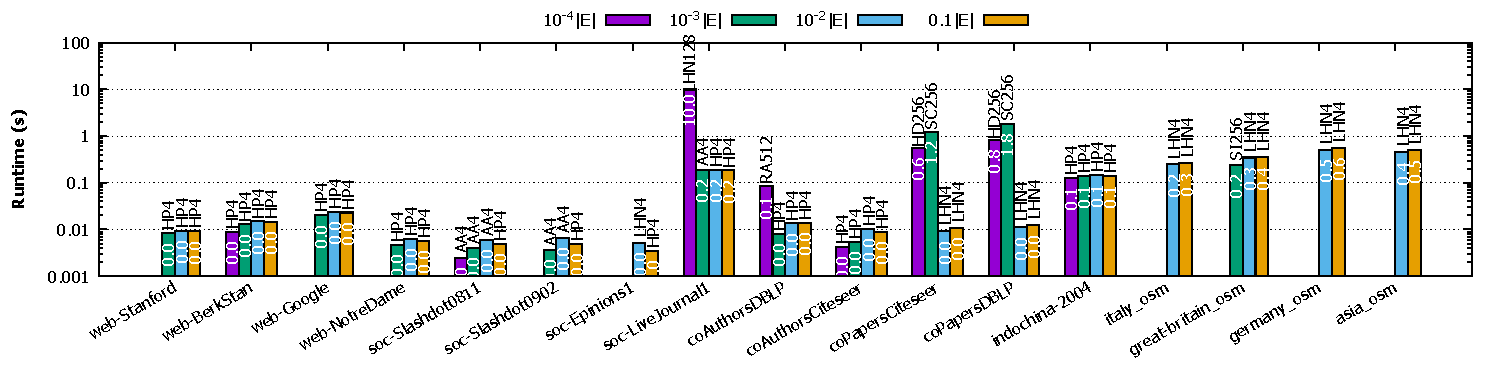
\includegraphics[width=0.98\linewidth]{out/input-small-runtime.pdf}
  }
  \subfigure[Precision]{
    \label{fig:input-small--precision}
    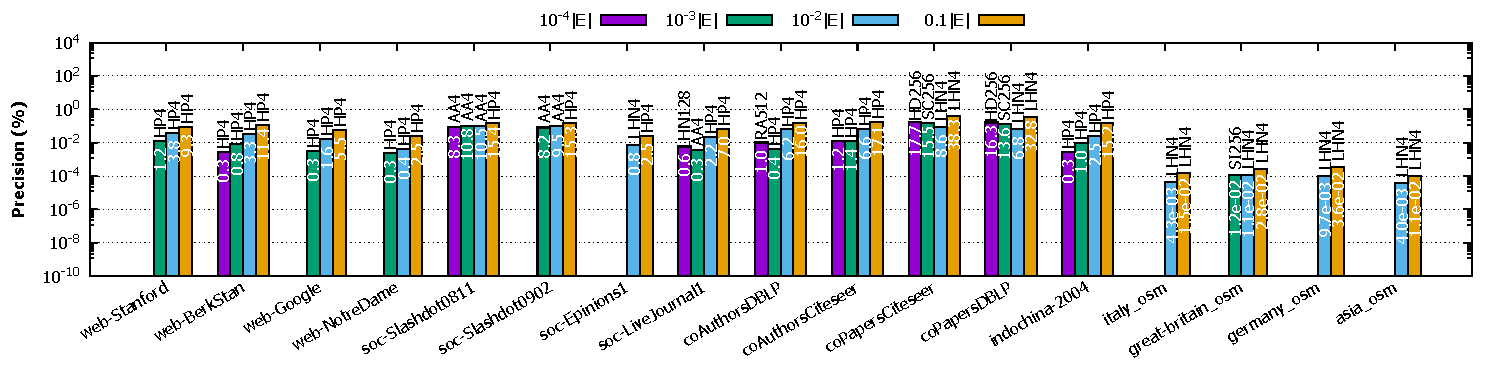
\includegraphics[width=0.98\linewidth]{out/input-small-precision.pdf}
  } \\[0ex]
  \caption{TODO. Input small.}
  \label{fig:input-small}
\end{figure*}

